\documentclass[annotation,times,page4]{itmo-student-thesis}

%% Опции пакета:
%% - annotation - если есть, генерируется аннотация, иначе не генерируется
%% - times - делает все шрифтом Times New Roman, требует пакета pscyr.
%% - page4 - начинает нумерацию оглавления с четвертой, а не с третьей страницы

%% Данные пакеты необязательны к использованию в бакалаврских/магистерских
%% Они нужны для иллюстративных целей
%% Начало
\usepackage{tikz}
\usetikzlibrary{arrows}
\usepackage{filecontents}
\begin{filecontents}{master-thesis.bib}
@inproceedings{ example-english,
    year        = {2016},
    booktitle   = {Proceedings of IEEE Congress on Evolutionary Computation},
    author      = {Maxim Buzdalov and Anatoly Shalyto},
    title       = {Hard Test Generation for Augmenting Path Maximum Flow 
                   Algorithms using Genetic Algorithms: Revisited},
    pages       = {2121-2128},
    langid      = {english}
}

@article{ example-russian,
    author      = {Максим Викторович Буздалов},
    title       = {Генерация тестов для олимпиадных задач по программированию 
                   с использованием генетических алгоритмов},
    journal     = {Научно-технический вестник {СПбГУ} {ИТМО}},
    number      = {2(72)},
    year        = {2011},
    pages       = {72-77},
    langid      = {russian}
}
\end{filecontents}
%% Конец

%% Указываем файл с библиографией.
\addbibresource{master-thesis.bib}

\begin{document}

\studygroup{М4238}
\title{Выделение групп пользователей в социльных медиа по их интересам и поведению на основе множества истоников данных}
\author{Дмитриев С.С.}
\supervisor{Фильченков А.А.}
\supervisordegree{кандидат. техн. наук, доцент}
\publishyear{2016}

%% Транслируется в "Направление и задача исследований"
\researchdirections{Целью данного исследования является создание алгоритма выделения групп пользователей социальных сетей на основе их социальных связей и поведения в социальных сетях}

%% Транслируется в "Проектная и исследовательская часть"
\researchpart{В рамках данной работы предложен подход, позволяющий выделять подгруппы у выбранной группы пользователей в социальных сетях, основывающийся на социальных связах и видимом поведении на публичных страницах. В основе предложенного подхода лежат несколько методов и концепций: представление социальных связей в виде графа, случайные марковские поля, а так же семантический анализ. В качестве примера использования подхода взята группа футбольных болельщиков, и подгруппа радикальных футбольных болельщиков, а так же группа феменисток и подгруппа радикальных феменисток. Были использованы данные пользователей из социальной сети Vk.com. Достигнуты следущие показатели для группы футбольных болельщиков: ; для группы феменисток: . Данный подход нов и так же может применятся для других групп и подгрупп пользователей.}

%% Транслируется в "Экономическая часть"
\economicpart{Данная работа не прополагает извлечения экономической выгоды из полученных результатов}

%% Транслируется в "Характеристика вопросов экологии, техники безопасности"
\ecologypart{Результатом работы является программный продукт, не нарушающий 
требования экологической безопасности.}

%% Транслируется в "Новизна полученных результатов"
\novelty{В рамках описываемого исследования представлен подход позволяющий опредлять принадлежность пользователя к определенной группе на основе его социальных связей и публичного поведения в социальной сети. Полученный подход является способом построения модели, не применявшимся для решения подобной задачи ранее. }

%% Транслируется в "Является ли работа продолжением курсовых проектов, есть ли публикации"
\cwpublications{Работа не является продолжением курсовых проектов. На тему диссертации имеются публикации. //СПИСОК-2016//... потом дописать}

%% Транслируется в "Практическая ценность работы. Рекомендации по внедрению"
\practicalimplications{Полученный алгоритм дает возможность определить является ли член выбранной группы так же членом её подможества. Это может быть использовано правоохранительными органами, т.к. алгоритм позволяет выделить, например подгруппы, склонные к бандитизму, пользователей потенциально более способных на совершение незаконных действий, нежели среднестатистический пользователь. Так же алгоритм может быть использован для усовершенствования таргетированной рекламы, например для выделения подгруппы фанатов определенного брэнда из группы его покупаетелей.}

%% Эта команда генерирует титульный лист и аннотацию.
\makemastertitle

%% Оглавление
\tableofcontents

%% Макрос для введения. Совместим со старым стилевиком.
\startprefacepage

Последнее время социальные медиа набрали огромную популярность. Такие сайты как Facebook.com, Vk.com, Twitter.com, обладают огромной аудиторией. Совокупный размер аудитории существующих социальных сетей составляет более двух миллиардов пользователей и их число постоянно растет. Они создают огромные массы контента, состоящего из их мнений и точек зрения. Так в течении суток на Facebook.com более 4.5 миллиардов раз пользователи ставят лайки, оставляют более 700 тысяч публичных комментариев, публикуют более 100 миллионов фотографий. Однако содержание этой информации в основном остается не исползованным. Тогда как оно может быть крайне важным.

Такие данные могут быть использованы для определения интересов, предпочтений и иных личных свойств пользователя. Часть подобной информации, пол, возраст,  местоположение, увлечения, может быть указана в профиле пользователя. Однако, зачастую, таки данные могут быть неполными, а иногда и неверными. А некоторые признаки, например, вероисповедание, политические взгляды или же принадлежность к неким общественным движениям обычно опускаются. Из-за этой неполноты возникает задача восстановления информации о пользователе.

Получение таких данных может быть полезна как бизнесу, так и государству. Используя восстановленные характеристики, можно уточнять таргетированную рекламу. Имея дополнительные данные об увлечениях людей, можно определять возможных преступников, что позволит предотвращать возможные нарушения или же прогнозировать конфликты.

Существует множество исследований о восстановлении данных, явно неуказанных в профилях пользователей. В них показано, что на основе информации о пользователе, его поведении в социльном медиа, можно с высокой точностью восстановить некоторые характеристики. 
Отдельной задачей стоит определения принадлежности ползователя к определенной группе, такой как, например, группа консерваторов или же группа любителей продукции Apple. Для решения  этой задачи часто используют данные о социальных связях пользователей. Показано, что они влияют на поведение человека, на его взгляды. 

В описываемом исследовании представлен подход для выделения подгруппы пользователей из определенной группы пользователей. Работа предложенного алогритма продемонстрирована на нескольких примерах: выделения подгруппы радикальных футбольных фанатов из группы футбольных болельщиков и выделения подгруппы радикальных фементисток из группы феменисток. Предпологается, что описываемый подход может быть использован на других группах и подгруппах пользователей различных социальных медиа.

%% Начало содержательной части.
\chapter{Обзор предметной области}
В данной главе описаны основные понятия, использующиеся в предметной области.

В разделе 1.1 описана задача о восстановлении характеристик пользователя, основные трудности, возникакающие при решении этой задачи. 

В разделе 1.2 рассмотрена задача о разделении пользователей на группы, определения их принадлежности к подгруппам.

В разделе 1.3 разобраны существующие методы и решения, полученные результаты в разнообразных исследованиях, посвещенных выделению групп пользователей.

В разделе 1.4 представлено формальное описание задачи, исследуемой в данной работе.

\section{Задача восстановления характеристик пользователя}
Задача о восстановлении характеристик пользователя, она же задача о профилировании пользователей, заключается в определении неизвестных характеристик пользователя, на основе имеющихся данных с определенных ресурсов. Под ресурсами подразумеваюстя как социальные медиа, так и любые другие сайты, обладающие системой регистрации, так же данные могут собираться одновременно с нескольких ресурсов.

Проблема восстановления часто встречается при необязательности заполнения некоторых полей. Часто необязательно заполнять пол, возраст, физические данные, тогда как эти данные могут быть очень важны для определенного рода ресурсов. Вычисление этой информации дает возможность улучшить качество таргетированных сервисов.

В социальных сетях зачастую указывается вовсе неверная информация, например, относительно возраста. Так появляется подтип задачи восстановления ~--- определение ошибочных свойств пользователя и восстановление как неизсвестных.

Помимо широко используемых характеристик пользователя, некоторые исследования посвещены таким задачам, как определение хронотипов пользователей. Данные о биоритмах людей полезны врачам и рекрутерам, оценивающим подойдет ли выбранный человек на определенную должность.

Существуют исследования определяющие психотип пользователя, используя лишь данные о них из их же аккаунтов с социальных медиа. Подобные исследования дают новые пути исследований для психологов.

Описанные задачи зачастую сводятся к задачи класстеризации, регрессии или классификации.

Однако так же многие из них можно свести к задаче о выделении групп пользователей.    

 
\section{Задача о выделении групп пользователей}
Задача о выделении групп пользователей является подтипом задачи о восттановлении характеристик пользователя. Она заключается в определеннии принадлежности выбранного пользователя к определенной группе, на основе имеющихся данных. 

Определение психотипа, хронотипа, задачи сводящиеся к выделению группы пользователей. Так, можно поставить задачу, как принадлежность пользователя к группе халериков, сангвиников, флегматиков, меланхоликов.

Ярким примером задачи о выделении групп пользователей может служить проблема определения принадлежности пользователя к политическому движению. В статьеописывается подход по определнию политических предпочтений пользователей. Исследователи предложили статистическую модель, в которой, в которой строится пространство идеологий, с построенными на них известными публичными сраницами в twitter, для которых была определена их идеалогия. Дальше в пространство помещались пользователи, их подписчики, координаты которых определялись исходя из их подписок.

Часто задачи о выделении групп пользователей решаются путем класстеризации пользователей.

В основе всех исследований по выделению групп пользователей лежат данные, на основе которых происходит восстановление информации. В основном это уже существующая информация из профилей пользователя. Так же часто используется информация из публичных сообщений, медиа-контент, такой как, видео, фотографии, музыка, социальные связи, поведение пользователя и т. д.

Главной проблемой в решении подобных задач является сведение задачи к математической модели. Приведение сырых данных к числовому виду так же зачастую бывает крайне непростой задачей.
  
\section{Обзор существующих решений}


\section{Постановка задачи настоящего исследования}
\section{Выводы по главе 1}

\chapter{Описание исследуемого подхода}
\section{Общая схема решения}
\section{Граф социальных связей}
\section{Определение тематики публичных сообщений}
%%\section{Латентный сементический анализ}
%%\section{Банальное решение задачи}
\section{Случайные марковские поля}
\section{Модифицированные случайные марковские поля}
\section{Выводы по главе 2}

\chapter{Реализация описаваемого подхода}
\section{Сбор данных}
\section{Использование алгоритмов}
\section{Способы измерения качества результата}
\section{Результаты}
\section{Выводы по главе 3}

\chapter{Заключение}
\chapter{Список исползованных источников}



В качестве примера таблицы приведена таблица~\ref{tab1}.

\begin{table}[!h]
\caption{Таблица умножения (фрагмент)}\label{tab1}
\centering
\begin{tabular}{|*{18}{c|}}\hline
-- & 1 & 2 & 3 & 4 & 5 & 6 & 7 & 8 & 9 & 10 & 11 & 12 & 13 & 14 & 15 & 16 & 17 \\\hline
1  & 1 & 2 & 3 & 4 & 5 & 6 & 7 & 8 & 9 & 10 & 11 & 12 & 13 & 14 & 15 & 16 & 17 \\\hline
2  & 2 & 4 & 6 & 8 & 10 & 12 & 14 & 16 & 18 & 20 & 22 & 24 & 26 & 28 & 30 & 32 & 34 \\\hline
3  & 3 & 6 & 9 & 12 & 15 & 18 & 21 & 24 & 27 & 30 & 33 & 36 & 39 & 42 & 45 & 48 & 51 \\\hline
4  & 4 & 8 & 12 & 16 & 20 & 24 & 28 & 32 & 36 & 40 & 44 & 48 & 52 & 56 & 60 & 64 & 68 \\\hline
\end{tabular}
\end{table}

Есть еще такое окружение \texttt{tabu}, его можно аккуратно растянуть на всю страницу.
Приведем пример (таблица~\ref{tab2}).

\begin{table}[!h]
\caption{Таблица умножения с помощью \texttt{tabu} (фрагмент)}\label{tab2}
\centering
\begin{tabu}{|*{18}{X[c]|}}\hline
-- & 1 & 2 & 3 & 4 & 5 & 6 & 7 & 8 & 9 & 10 & 11 & 12 & 13 & 14 & 15 & 16 & 17 \\\hline
1  & 1 & 2 & 3 & 4 & 5 & 6 & 7 & 8 & 9 & 10 & 11 & 12 & 13 & 14 & 15 & 16 & 17 \\\hline
2  & 2 & 4 & 6 & 8 & 10 & 12 & 14 & 16 & 18 & 20 & 22 & 24 & 26 & 28 & 30 & 32 & 34 \\\hline
3  & 3 & 6 & 9 & 12 & 15 & 18 & 21 & 24 & 27 & 30 & 33 & 36 & 39 & 42 & 45 & 48 & 51 \\\hline
4  & 4 & 8 & 12 & 16 & 20 & 24 & 28 & 32 & 36 & 40 & 44 & 48 & 52 & 56 & 60 & 64 & 68 \\\hline
\end{tabu}
\end{table}

пользователей различных социальных медиа.
пользователей различных социальных медиа.
пользователей различных социальных медиа.
\section{Рисунки}

Пример рисунка (c помощью \texttt{TikZ}) приведен на рисунке~\ref{fig1}. Под \texttt{pdflatex} можно также
использовать \texttt{*.jpg}, \texttt{*.png} и даже \texttt{*.pdf}, под \texttt{latex} можно использовать
Metapost. Последний можно использовать и под \texttt{pdflatex}, для чего в стилевике продекларированы
номера картинок от~1 до~20.

\begin{figure}[!h]
\caption{Пример рисунка}\label{fig1}
\centering
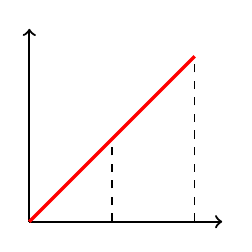
\begin{tikzpicture}[scale=0.7]
\draw[thick,->] (0,0)--(3.5,0);
\draw[thick,->] (0,0)--(0,3.5);
\draw[very thick, red] (0,0)--(3,3);
\draw[dashed] (3,0)--(3,3);
\draw[dashed] (1.5,0)--(1.5,1.5);
\end{tikzpicture}
\end{figure}

\section{Листинги}

В работах студентов кафедры <<Компьютерные технологии>> часто встречаются различные листинги. Листинги бывают
двух основных видов~--- исходный код и псевдокод. Первый оформляется с помощью окружения \texttt{lstlisting}
из пакета \texttt{listings}, который уже включается в стилевике и немного настроен. Пример Hello World на Java
приведен на листинге~\ref{lst1}.

\begin{lstlisting}[float=!h,caption={Пример исходного кода на Java},label={lst1}]
public class HelloWorld {
	public static void main(String[] args) {
		System.out.println("Hello, world!");
	}
}
\end{lstlisting}

Псевдокод можно оформлять с помощью разных пакетов. В данном стилевике включается пакет \texttt{algorithmicx}.
Сам по себе он не генерирует флоатов, поэтому для них используется пакет \texttt{algorithm}.
Пример их совместного использования приведен на листинге~\ref{lst2}. Обратите внимание, что флоаты разные, а 
нумерация~--- общая!

\begin{algorithm}[!h]
\caption{Пример псевдокода}\label{lst2}
\begin{algorithmic}
	\Function{IsPrime}{$N$}
		\For{$t \gets [2; \lfloor\sqrt{N}\rfloor]$}
			\If{$N \bmod t = 0$}
				\State\Return \textsc{false}
			\EndIf
		\EndFor
		\State\Return \textsc{true}
	\EndFunction
\end{algorithmic}
\end{algorithm}

Наконец, листинги из \texttt{listings} тоже можно подвешивать с помощью \texttt{algorithm},
пример на листинге~\ref{lst3}.

\begin{algorithm}[!h]
\caption{Исходный код и флоат \texttt{algorithm}}\label{lst3}
\begin{lstlisting}
public class HelloWorld {
	public static void main(String[] args) {
		System.out.println("Hello, world!");
	}
}
\end{lstlisting}
\end{algorithm}

\chapter{Проверка сквозной нумерации}

Листинг~\ref{lst4} должен иметь номер 4.

\begin{algorithm}[!h]
\caption{Исходный код и флоат \texttt{algorithm}}\label{lst4}
\begin{lstlisting}
public class HelloWorld {
	public static void main(String[] args) {
		System.out.println("Hello, world!");
	}
}
\end{lstlisting}
\end{algorithm}

Рисунок~\ref{fig2} должен иметь номер 2.

\begin{figure}[!h]
\caption{Пример рисунка}\label{fig2}
\centering
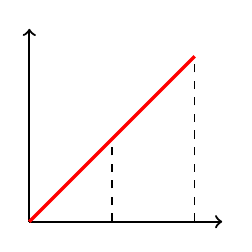
\begin{tikzpicture}[scale=0.7]
\draw[thick,->] (0,0)--(3.5,0);
\draw[thick,->] (0,0)--(0,3.5);
\draw[very thick, red] (0,0)--(3,3);
\draw[dashed] (3,0)--(3,3);
\draw[dashed] (1.5,0)--(1.5,1.5);
\end{tikzpicture}
\end{figure}

Таблица~\ref{tab3} должна иметь номер 3.

\begin{table}[!h]
\caption{Таблица умножения с помощью \texttt{tabu} (фрагмент)}\label{tab3}
\centering
\begin{tabu}{|*{18}{X[c]|}}\hline
-- & 1 & 2 & 3 & 4 & 5 & 6 & 7 & 8 & 9 & 10 & 11 & 12 & 13 & 14 & 15 & 16 & 17 \\\hline
1  & 1 & 2 & 3 & 4 & 5 & 6 & 7 & 8 & 9 & 10 & 11 & 12 & 13 & 14 & 15 & 16 & 17 \\\hline
2  & 2 & 4 & 6 & 8 & 10 & 12 & 14 & 16 & 18 & 20 & 22 & 24 & 26 & 28 & 30 & 32 & 34 \\\hline
3  & 3 & 6 & 9 & 12 & 15 & 18 & 21 & 24 & 27 & 30 & 33 & 36 & 39 & 42 & 45 & 48 & 51 \\\hline
4  & 4 & 8 & 12 & 16 & 20 & 24 & 28 & 32 & 36 & 40 & 44 & 48 & 52 & 56 & 60 & 64 & 68 \\\hline
\end{tabu}
\end{table}

\chapterconclusion

В конце каждой главы желательно делать выводы. Вывод по данной главе~--- нумерация работает корректно, ура!

%% Макрос для заключения. Совместим со старым стилевиком.
\startconclusionpage

В данном разделе размещается заключение.

%% Обратите внимание на heading. Без него тоже работает, но название будет другим.
\printbibliography[heading=trueHeading]

%% После этой команды chapter будет генерировать приложения, нумерованные русскими буквами.
%% \startappendices из старого стилевика будет делать то же самое
\appendix

\chapter{Пример приложения}

Пример ссылок на литературные источники: \cite{example-english, example-russian}.
\end{document}
